\documentclass[12pt]{article}
\usepackage{graphicx}
\usepackage{float}
\begin{document}
\title{Computer Science 145, Homework 5}
\date{March 6th, 2019}
\author{Michael Wu\\UID: 404751542}
\maketitle

\section*{Problem 1}

\paragraph{a)}

In the first iteration we obtain the following table.
\begin{center}
    \begin{tabular}{c|c}
        Item Set & Support \\
        \hline
        \(\{a\}\) & 6\\
        \(\{b\}\) & 8\\
        \(\{c\}\) & 6\\
        \(\{d\}\) & 4\\
        \(\{e\}\) & 2\\
        \(\{i\}\) & 1\\
        \(\{j\}\) & 1\\
        \(\{k\}\) & 1
    \end{tabular}
\end{center}
We can ignore \(\{i\}\), \(\{j\}\), and \(\{k\}\) since they are not frequent. Then we have the following length
two candidates and supports.
\begin{center}
    \begin{tabular}{c|c}
        Item Set & Support \\
        \hline
        \(\{a,b\}\) & 4\\
        \(\{a,c\}\) & 4\\
        \(\{a,d\}\) & 2\\
        \(\{a,e\}\) & 2\\
        \(\{b,c\}\) & 4\\
        \(\{b,d\}\) & 4\\
        \(\{b,e\}\) & 2\\
        \(\{c,d\}\) & 1\\
        \(\{c,e\}\) & 1\\
        \(\{d,e\}\) & 0\\
    \end{tabular}
\end{center}
We can ignore \(\{c,d\}\), \(\{c,e\}\), and \(\{d,e\}\) since they are not frequent. Then we generate the length three
candidates by looking at the length two frequent patterns and combining the ones that only differ in the last element.
During candidate generation we can prune \(\{a,c,d\}\), \(\{a,c,e\}\), \(\{a,d,e\}\), \(\{b,c,d\}\), \(\{b,c,e\}\),
and \(\{b,d,e\}\) since they are supersets of the previous length two sets that are not frequent. We
then have the following length three candidates and supports.
\begin{center}
    \begin{tabular}{c|c}
        Item Set & Support \\
        \hline
        \(\{a,b,c\}\) & 2\\
        \(\{a,b,d\}\) & 2\\
        \(\{a,b,e\}\) & 2
    \end{tabular}
\end{center}
During generation of length four candidates, we will prune away all the candidates because they contain one of \(\{c,d\}\),
\(\{c,e\}\), or \(\{d,e\}\) which are not frequent. Thus our frequent patterns are
\[\{a,b,c\}, \{a,b,d\}, \{a,b,e\}\]
and any subset of these item sets.

\paragraph{b)}

Our initial F-list contains \(a\) to \(e\). If we arrange by frequency the list becomes \(\{b,a,c,d,e\}\). The ordered
frequent items in the database are shown in the following table.
\begin{center}
    \begin{tabular}{c|c}
        TID & Ordered Frequent Items\\
        \hline
        1 & \{b,c\}\\
        2 & \{b,a,d\}\\
        3 & \{a,c\}\\
        4 & \{b,d\}\\
        5 & \{b,a,c,e\}\\
        6 & \{b,c\}\\
        7 & \{a,c\}\\
        8 & \{b,a,e\}\\
        9 & \{b,d\}\\
        10 & \{b,a,c,d\}
    \end{tabular}
\end{center}
The FP-tree is shown below.
\begin{figure}[H]
    \begin{center}
        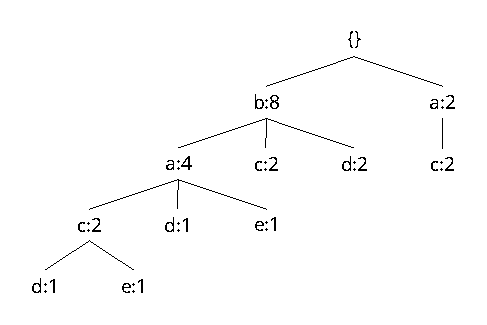
\includegraphics[width=4.5in]{problem1b.pdf}
    \end{center}
\end{figure}

\paragraph{c)}

The conditional pattern base for \(d\) is \(\{bac:1, ba:1, b:2\}\). We can see that only \(b\) and \(a\) are
frequent here, so the conditional FP-tree is the one shown below.
\begin{figure}[H]
    \begin{center}
        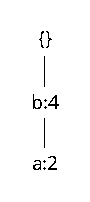
\includegraphics[width=1in]{problem1c.pdf}
    \end{center}
\end{figure}

\paragraph{d)}

Based on the conditional FP-tree we have the frequent patterns \(\{bad:2, ad:2, bd:4, d:4\}\).

\section*{Problem 2}

\paragraph{a)}

\paragraph{b)}

\paragraph{c)}

\section*{Problem 3}

\paragraph{a)}

\paragraph{b)}

\section*{Problem 4}

\paragraph{a)}

This contains six elements. The length of \(s\) is eight. It contains \(2^6-1=63\) non-empty subsequences.

\paragraph{b)}

\end{document}